\documentclass[a4paper]{scrreprt}

%% Language and font encodings
\usepackage[english]{babel}
\usepackage[utf8x]{inputenc}
\usepackage[T1]{fontenc}
\usepackage{eurosym}

%% Sets page size and margins
\usepackage[a4paper,top=3cm,bottom=2cm,left=3cm,right=3cm,marginparwidth=1.75cm]{geometry}

%% Useful packages
\usepackage{amsmath}
\usepackage{graphicx}
\usepackage[colorinlistoftodos]{todonotes}
\usepackage[colorlinks=true, allcolors=blue]{hyperref}


\usepackage{comment}
\title{The Tourist}
\subtitle{"Super Mario Bros. 3, but based in Graz and 100\% satire"}
\author{Michelic Florian \\ Perz Markus \\ Ribeiro Skreinig Lucchas\\ Ruprecht Irena \\ Tschuden Julia}


\begin{document}
\maketitle

\null\vfill
\noindent
Game Design Document Template\\ 
Version v1.1, Nov 2016\\
Version v1.2, Dec 2017\\
Version v1.3, Nov 2019\\
Copyright 2017-2019 - Johanna Pirker \#tugamedev\\
\newpage

\begin{abstract}
\noindent You are a tourist and you need to survive your stay in Graz. Fight enemies and find your way through Graz to obtain selfies, while discovering the most charming city of Austria.
Meet typical Grazer inhabitants like hipsters, snobs and of course zombies. 
Wear fancy outfits to make your selfies really pop. Consume traditional Grazer snacks like the infamous "Frankfurter with Semmel" or "Geidorfer" beer to get the most out the city. Get to know the dynamic environment you will use to overcome obstacles. But most importantly - enjoy your stay.
\newline

\end{abstract}

\tableofcontents

% ______________________
% chapter Overview - Rena
% ______________________
\chapter{Overview}

\begin{comment}
Main features and aspects of your game on a first page, describing story elements. -> "selling page", publisher should be able to decide after reading this single page whether to buy in or not 
\end{comment}

\section{Main Concept}
%%describe you main concept in one paragraph
A classical side-scrolling 2D-platformer featuring stereotypical characters and items that humorously relate to the City of Graz. The player's character is a tourist arriving at the main train station in Graz. The goal is to collect selfies from typical tourist attractions. These attractions form the goals of the different stages, which the player has to master in order to receive a selfie as reward.
Once all selfies are collected, the tourists business in Graz could be considered done. Unless of course the tourist is up for another sightseeing round-trip in the dynamic city of Graz. 

\section{Unique Selling Point}
A humorous take on our hometown combined with classical gameplay mechanics everyone knows and has loved since the \textit{Super Mario} series. In the undergrounds of Graz, however, everything is dynamic and simulated so that one simple action may snowball into a series of events the player may not have foreseen. 
\\ The hand-crafted art and sprites are all based on things one might take for granted, but that uniquely shape Graz into the city we know so well.


% ______________________
% chapter References - Luke
% ______________________

\chapter{References} 
Our game's core features include 2D side-scrolling platformer movement paired with 2D side-scrolling brawler combat. Additionally, the game features a playable character with an individually customizable head, torso, and legs. \\ \\
Similar games are:

\begin{itemize}
\item Super Mario Bros. 3
\item Zelda 2: The Adventure of Link
\item Streets of Rage
\item Heave Ho
\end{itemize}


% ______________________
% chapter Specification and Market Analysis - Jules
% ______________________

\chapter{Specification}

\section{Player(s) / Target-group}
%\textit{who is the target group?}\\
Our major target group are people (all gender identities) living in Graz, between the ages of 18 and 34 years. Our players are casual or hardcore players, who value and accept the humor in the game's presentation and world building, e.g. enemies being portrayed by stereotypical Grazer residents. In addition our players are fond of solving the platform maze which is represented by different parts of Graz. \\\\
Another target group are tourists and exchange students, who might want to see Graz from a different side. This target group also mostly consists of younger people.

\section{Genre}
%\textit{what is the genre of the game?}\\
The genre of our game is Platformer/Brawler.

\section{Art Style}
%\textit{the art style of the game?}\\
For the background assets we chose a semi-realistic and modern art style. For the main character and enemies a cartoonish and modern art stlye was used. All of our graphics are hand-crafted by our artists.

\section{Forms of Engagement}
Thinking of Hunicke's kinds of "fun", our game focuses on the highlighted aspects below.
\newline
\begin{itemize}
  \item \textbf{1. Sensation - Game as sense-pleasure} 
  \item 2. Fantasy - Game as make-believe
  \item 3. Narrative - Game as drama
  \item \textbf{4. Challenge - Game as obstacle course}
  \item 5. Fellowship -  Game as social framework
  \item \textbf{6. Discovery - Game as uncharted territory }
  \item 7. Expression - Game as self-discovery 
  \item 8. Submission - Game as pastime
\end{itemize}
We will focus on making the game challenging as well as sensational. Players should enjoy to struggle through levels while discovering known locations in our version of Graz.

% ______________________
% chapter Game Details - Markus
% ______________________


\chapter{Gameplay and Game Setting}
%\textit{be specific about the core game features } \\
"Super Mario, but based in Graz and 100\% satire" is a more than accurate description of the game. Even though the style may differ, the overall gameplay will quickly remind the player of the classic game featuring the italian plumber, while still bringing a new and fresh tone to the formula. 
\noindent It should be fun and challenging to play a platformer like Mario in Graz, where NPCs, collectables, items, effects and locations reflect the general flair of Styria's capitol city.

\section{Mood and Emotions}

Concerning emotions, our game mainly creates fun and comedy because our game displays an ironic, self-deprecating, oversimplified image of Graz, as told by Grazers, but observed by a non-Grazer. In addition our game encourages the user to be ambitious by featuring a challenging level design.

\section{Story}
%\textit{the story of the game} \\

The game tells the story of a first-time tourist in Graz, struggling to find his way through the city. While the drive to get selfies in front of the important places in Graz pushes the tourist to visit all corners of Graz, this odyssey is way more challenging than typical sight-seeing trips.

\section{World/Environment}

The game takes place in Graz. As soon as the main character arrives at the central station the player can navigate to different places by choosing the right station. The levels themselves are a simplified 2D representation of the current street/place/setting in Graz that fit the style of our game. \\

\noindent Currently our games features the following levels:
\begin{itemize}
    \item Tutorial
    \item Hauptplatz (easy)
    \item Schlossberg (hard)
    \item Kusthaus (medium)
    \item Stadthalle (medium)
    \item Oper (easy)
    \item Zentralfriedhof (hard)
    
\end{itemize}

\section{Objects in the Game}
%\textit{what objects will be in the game?} \\

The set of interactable game objects consists of consumable and environmental objects. The following consumable items are available in the game:

\begin{itemize}
\item Döner (increases punch damage and force)
\item Geidorfer beer (increases move and attack speed)
\item Frankfurter + Semmel(=bread roll) (regenerates health)
\item Collectable selfies
\end{itemize}

The movable environmental objects help the player to overcome heights or other puzzle key spots. There are solid heavy objects such as garbage containers or cars as well as bouncy objects such as couches and parasols. The persistent objects in the levels are balconies the player can jump on and the simulated platforms. These moving platforms behave individually and have different attributes such as "load capacity".



\section{Characters in the Game}
%\textit{who are the characters in the game?}\\

The main character is a male, customizable tourist, who is new to Graz.\\
The following NPCs/enemies may show up during the tourists journey:
\begin{itemize}
\item Zombies
\item Snobs (economics students)
\item Hobos
\item Hipster
\item Hooligans
\end{itemize}

The individual characteristics manifest themselves in varying attack speed, movement and motion. Hobos for instance will move around quite randomly, while a Hooligan may run directly towards the player to satisfy his craving for a fist fight.

\section{Main Objective}
%\textit{what is the goal / main objective of the game?}

The player shall visit different attractions and famous places in Graz, without dying during the levels. After each attraction the player shall be rewarded with his own, unique selfie at the place. To succeed and finish the game the player should make selfies at each setting in Graz. To achieve the main goal, the player can empower themself with consumable items. 

\section{Core Mechanics}
%\textit{very important section: what are the core mechanics? be specific}\\

The game is a level based game where the player faces different challenges in the individual levels, be it platforming challenges or difficulty spikes during the combat sections. The levels can be solved by interacting with the game environment using the following controls:

\section{Controls}
\begin{itemize}
    \item Left/Right arrows for horizontal movement
    \item Space bar to jump
    \item Q button to hit objects/fight enemies
    \item R button to grab objects
    \item 3 button to use Frankfurter
    \item 2 button to use Beer
    \item 1 button to use Doener
    \item Return button to restart the level
\end{itemize}


% ______________________
% chapter Front End - Jules
% ______________________


\chapter{Front End}
%\textit{description of front end such as start screen, menu screens,.. } 

\section{Start Screen}
The start screen features the games name, as well as a message, which tells the player to press a random key to enter the game.

\section{Menus}

As seen in Figure~\ref{fig:menu}, our game has the following menus:
\begin{itemize}
\item Start Game
\item Tutorial
\item Gallery
\item Credits
\item Quit
\end{itemize}

\begin{figure}[h]
\centering
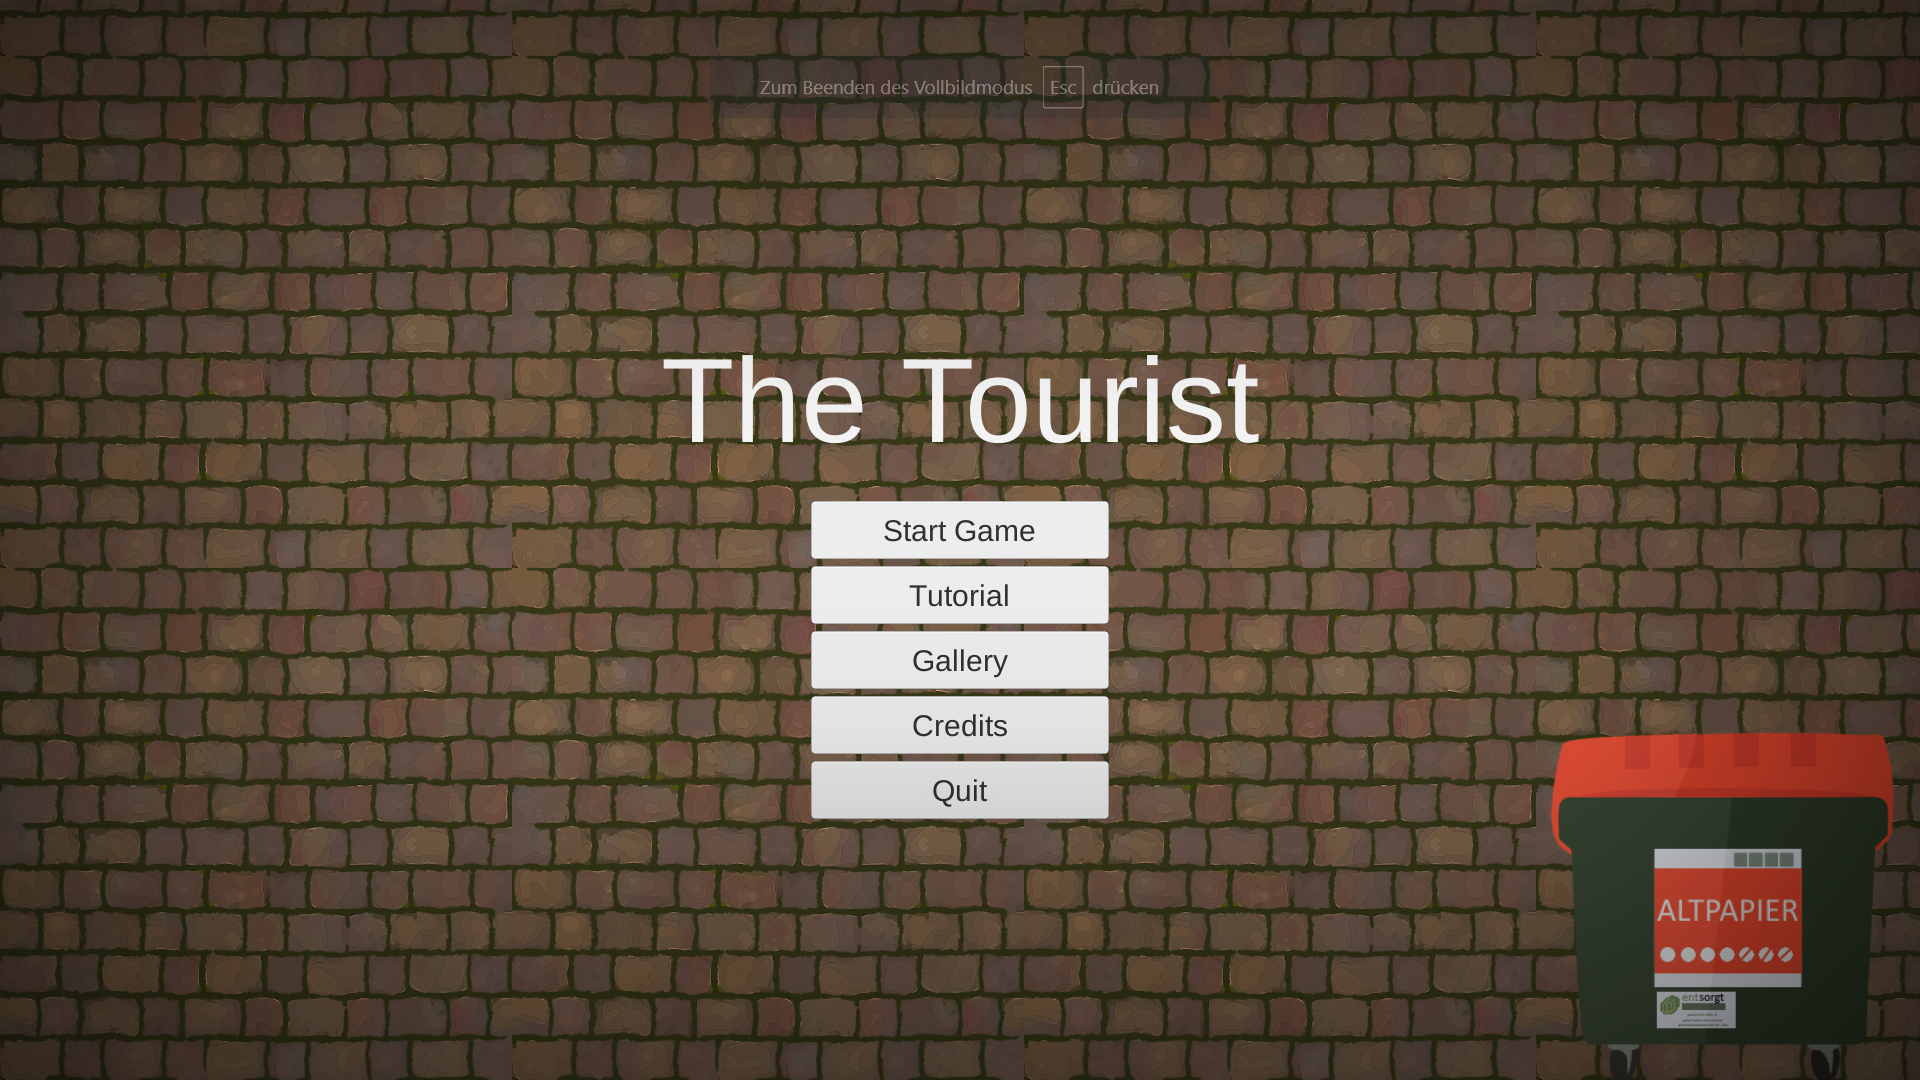
\includegraphics[width=0.6\textwidth]{menu.png}
\caption{The game's menu with all of its items.}
\label{fig:menu}
\end{figure}

\noindent After the start screen the \textbf{Menu} (see Figure~\ref{fig:menu}) is displayed. The menu item \textbf{Start Game} brings the main character to the central station, where the player can navigate to different stops to start the individual levels. Additionally, the central station includes a dressing room (see Figure~\ref{fig:char}), where the outfit of the main character can be changed and a photo lab, where the gallery can be viewed in-game (see Figure~\ref{fig:gallery}).
The menu item \textbf{Tutorial} starts the tutorial, where the player can get in touch with the controls. The menu item \textbf{Gallery} displays all the selfies the player achieved during their playthrough. The menu item \textbf{Credits} lists the creators of this game. The menu item \textbf{Quit} quits the game.



\begin{figure}[h]
\centering
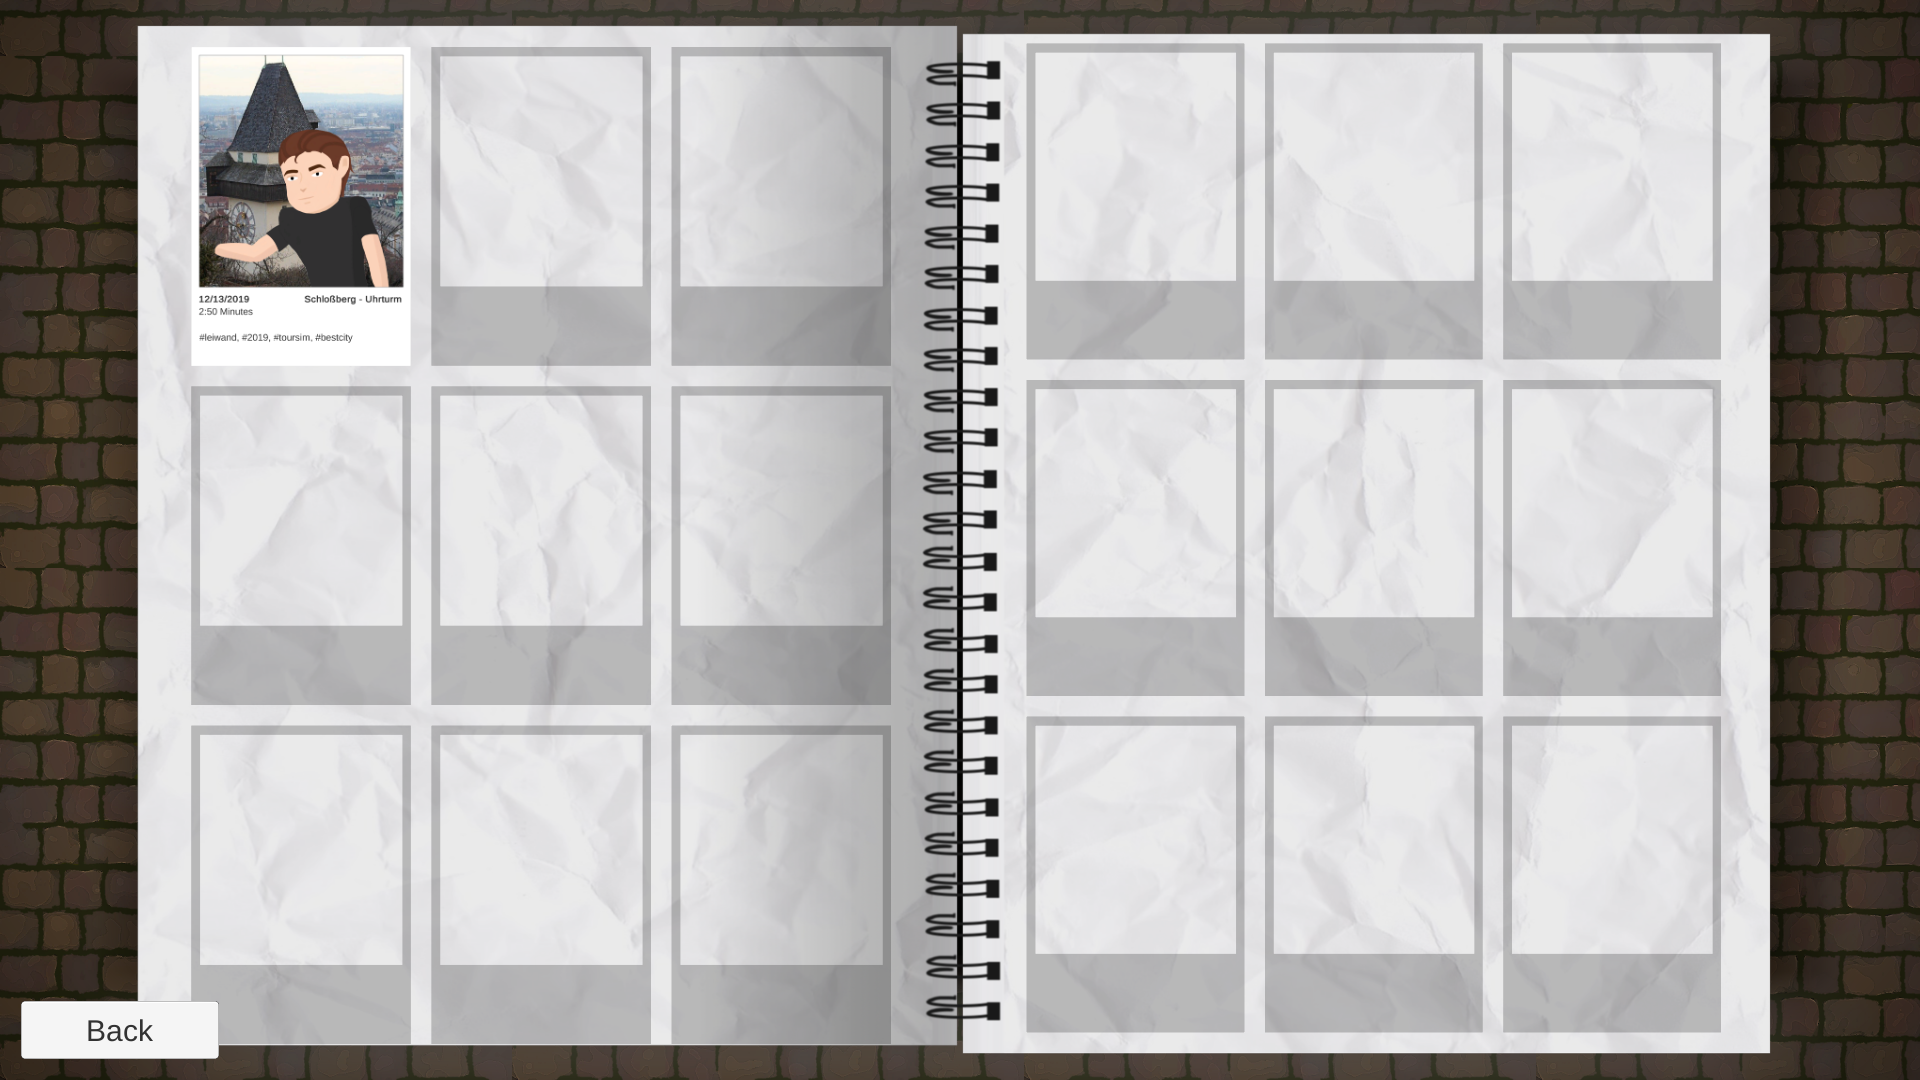
\includegraphics[width=0.6\textwidth]{gallery.png}
\caption{The gallery, where all obtained selfies can be seen.}
\label{fig:gallery}
\end{figure}

\begin{figure}[h]
\centering
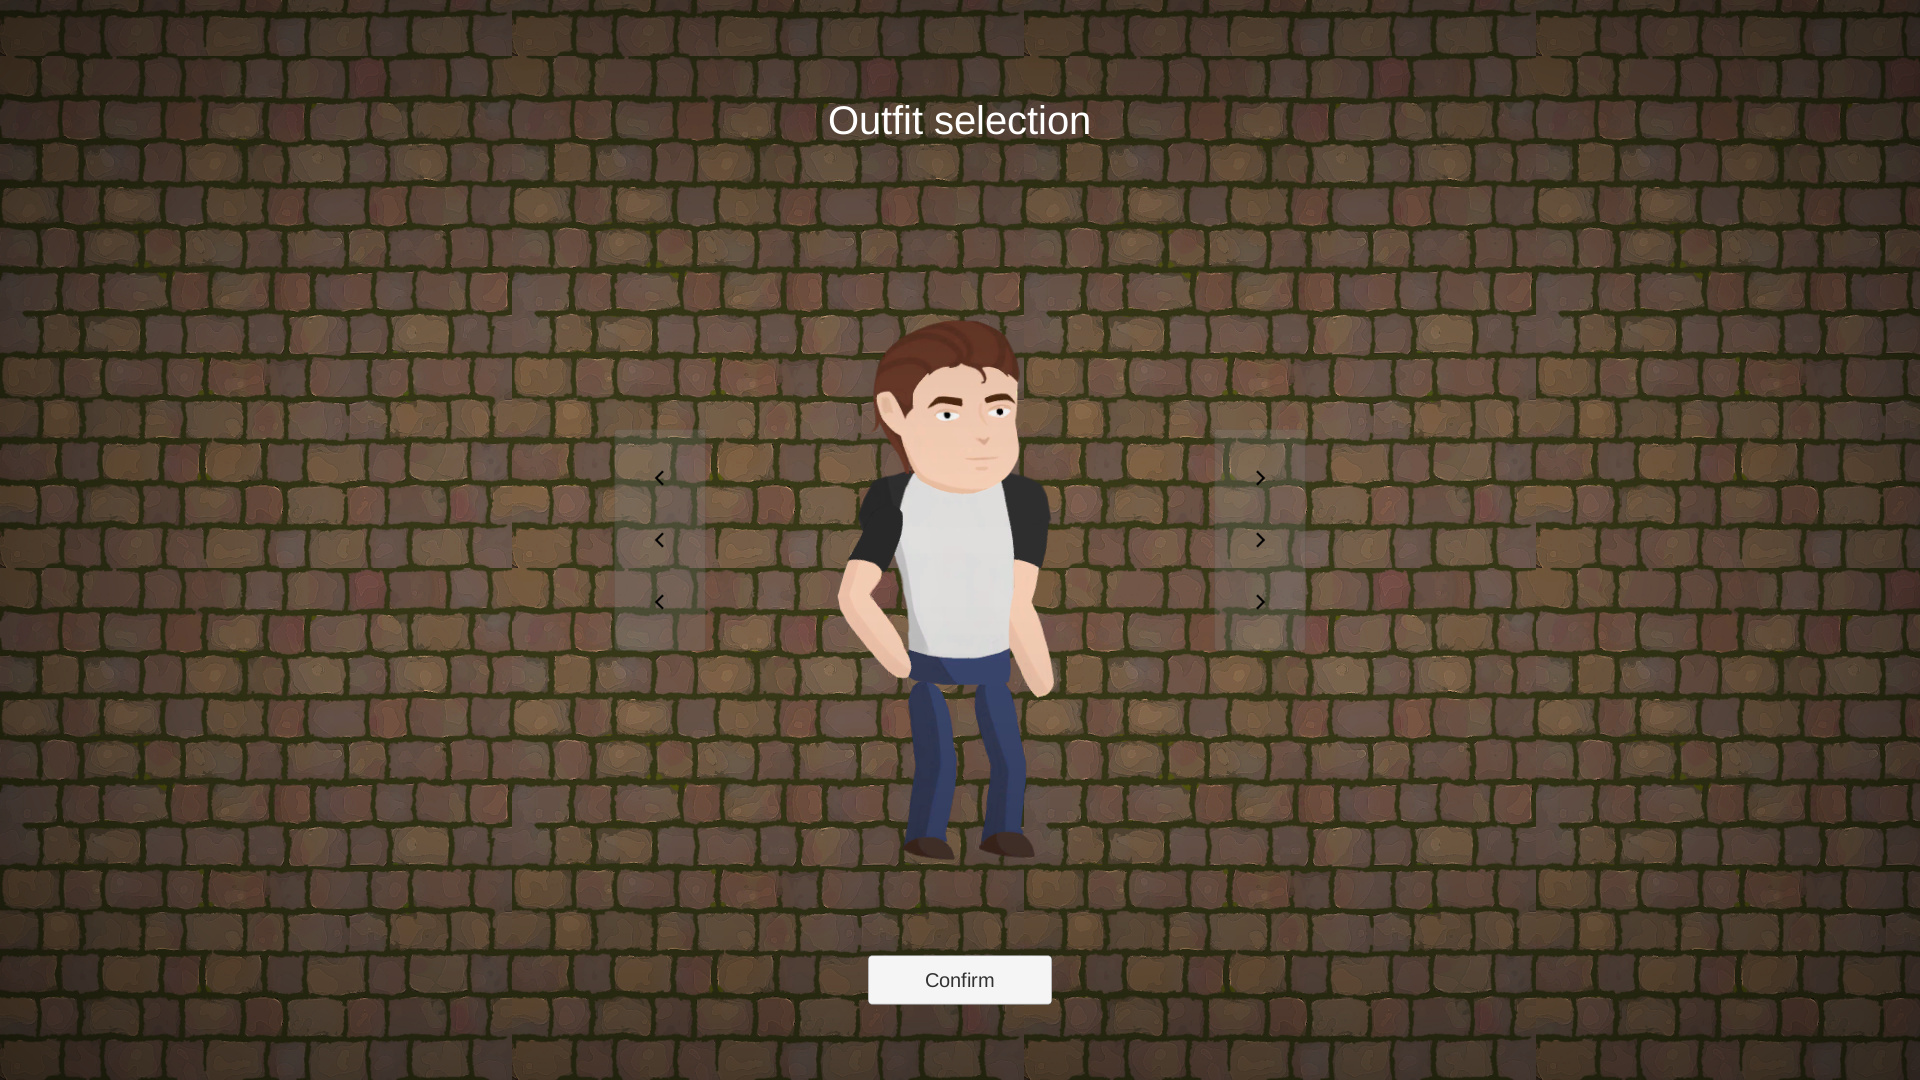
\includegraphics[width=0.6\textwidth]{dressing.png}
\caption{The dressing room, where the outfit can be changed.}
\label{fig:char}
\end{figure}



% ______________________
% chapter Game Details - all
% ______________________

\chapter{Technology}

\section{Target Systems}
The game is targeted to run on PCs.

\section{Hardware}
The game supports keyboard interfaces.

\section{Development Systems/Tools}
\begin{itemize}
    \item \textbf{Game engine:} Unity
    \item \textbf{IDE/Editors:} Visual Studio, VS Code, Sublime, Google Sheets
    \item \textbf{Image/Asset manipulation:} AutoDesk SketchBook, Adobe Photoshop CS6, Adobe Photoshop CC 2015, Paint.NET
    \item \textbf{Sound editing:} Audacity
\end{itemize}

% ______________________
% chapter Topic and Inclusion - Luke
% ______________________

\chapter{Topic and Inclusion }

%describe here how you plan to address the main topic (main theme) and the 

\section{Main Theme}
The theme of Graz is baked into the very core of the game. The setting of the game is a representation of the city of Graz, the objective concerns Graz' signature landmarks, and the characters and items are all symbolic of day-to-day Grazer life.
\section{Inclusion}
The game does not exclude any player, given the ability to read and use classic control schemes such as a keyboard.
\subsection{Diversity}
Since our main focus does not lie on diversity we did not address this topic.
\subsection{Accessibility}
The game is not designed for any player with particular motor impairments or visual disabilities, however impairments such as color blindness or deafness should not hinder anyone's ability to play or enjoy the game.
\subsection{Humanity}
The game has some examples of dark humor, which might be offensive to some, however the intention is purely comedic and shouldn't deeply conflict with anyone's moral alignment.

% ______________________
% chapter Marketing and Publishing Strategy - Flo
% ______________________


\chapter{Marketing and Publishing Strategy}
 
 \begin{itemize}
     \item \textbf{Social Media:} We may present our game on common social media platforms. People could follow us, discuss our game and share ideas which may find their way into the final product. 
     \item \textbf{Youtubers/Streamers:} To get attention for our social media appearance,
we may send a free WebGL-Demo to various Youtubers/Streamers.
    \item \textbf{Local Media:} Local media institutions may be contacted, since they might could interested in the satiric aspect of the game.
    \item \textbf{Gaming events:} We may attend game related events in the area to showcase and promote our game.
 \end{itemize}

% ______________________
% chapter Game Details
% ______________________

\chapter{Timeline and Cost Estimation}

\begin{table}[h]
\centering
\begin{tabular}{|l|l|l|}
\hline
Milestone & Description & Date \\\hline
& Official Start Date & 01.12.2019 \\
1 & First prototypical level  & 15.12.2019 \\
2 & Menu working  & 29.12.2019 \\
3 & 20\% of the levels working  & 29.12.2019 \\
4 & Items working  & 12.01.2020 \\
5 & 40\% of the levels working  & 12.01.2020 \\
6 & Graphics and effects working  & 26.01.2020 \\
7 & 60\% of the levels working  & 26.01.2020 \\
8 & Sounds, refined gameplay mechanics & 09.02.2020 \\
9 & 80\% of the levels working  & 09.02.2020 \\
10 & All levels working  & 23.02.2020 \\
11 & Balancing  & 01.03.2020 \\
& End of Project & 06.03.2020 \\
\hline
\end{tabular}
\caption{\label{tab:schedule} Schedule}
\end{table}

\section{Time Estimation}
As seen in Table~\ref{tab:schedule}, our team plans to finish the game by 06.03.2020. Each team member will invest 8 hours a week into this game, which results in a total of 480 hours. We plan to use 10\% of this time for organisational procedures, e.g. discussing our plans and process. The remaining 90\% will be dedicated to the game development and content creation. 

\section{Cost Estimation}
After considering the expected duration of our project, we plan to use \textbf{15.000 {\euro}} in total. This is divided up as follows: 9.000 {\euro} will make up our salaries, 1.000 {\euro} will be used for user studies and evaluation while the remaining 4.000 {\euro} will serve as marketing budget. 


% ______________________
% chapter Game Details
% ______________________


\chapter{Team and Credits}
\begin{comment}
\textit{most important - who are you, who takes what role?} \\
\end{comment}
\begin{itemize}
    \item \textbf{Project Management:} Julia
    \item \textbf{Programming:} Florian, Markus, Irena
    \item \textbf{Art Design, Animation:} Julia, Lucchas
    \item \textbf{Level Design:} Florian, Markus, Irena
    
\end{itemize}

\textbf{Copyrights of thirdparty images:}
\begin{itemize}

\item Hauptplatz: CC by Isiwal on Wikipedia 
\item Zentralfriedhof: CC by Tokfo on Wikipedia 
\item Stadthalle: CC by Jacktd on Wikipedia 
\item Other polaroids: C by justgrazthings on Instagram 

\end{itemize}

\textbf{Sounds: } \url{https://www.freesound.org/} \newline

\textbf{Textures: } \url{https://www.textures.com/} \newline



%\todo[inline, color=green!40]{This is an inline comment.}

%\bibliographystyle{alpha}
%\bibliography{sample}

\end{document}